\documentclass%[handout]%
{beamer}
%\usetheme{Execushares}
\usetheme{AnnArbor}
\usecolortheme{beaver}
%\setbeamercolor{title}{parent=structure,bg=green!50!black,fg=white}
%\usecolortheme{dolphin}
\setbeamertemplate{navigation symbols}{}%remove navigation symbols

\usepackage{amsmath}
\usepackage{amssymb}
\usepackage{amsthm}
%\usepackage[utf8]{inputenc}
\usepackage[czech]{babel}
\usepackage{tikz-cd}
\usepackage[mathscr]{euscript}
\usepackage[IL2]{fontenc}
\usepackage{mathtools}
\usepackage[normalem]{ulem}

\usetikzlibrary{calc,shapes.callouts,shapes.arrows}

%\usepackage{beamerarticle}

%\usepackage{bbm}

\def\rllap#1{\hbox to0pt{\hss#1\hss}}

%\newcommand{\bubblethis}[2]{
        %\tikz[remember picture,baseline]{\node[anchor=base,inner sep=0,outer sep=0]%
        %(#1) {\underline{#1}};\node[overlay,cloud callout,callout relative pointer={(-0.2cm,+0.7cm)},%
        %aspect=2.5,fill=yellow!90] at ($(#1.north)+(-0.5cm,1.6cm)$) {#2};}%
    %}%
		%
%\newcommand{\speechthis}[2]{
        %\tikz[remember picture,baseline]{\node[anchor=base,inner sep=0,outer sep=0]%
        %(pom) {#1};\node[overlay,ellipse callout,fill=blue!50] 
        %at ($(pom.north)+(1cm,+0.8cm)$) {#2};}%
    %}%
		
\newcommand{\R}{\mathbb R}

\title{Limity funkcí}
\author{Alexander Slávik} %  and J. Trlifaj
\subtitle{Jednostranné limity}
\institute{Gymnázium Voděradská}
\date{4. 11. 2020}

\begin{document}

%
%\frame{\titlepage}

%
%\begin{frame}
	%\frametitle{Limita složené funkce}
	%
	%\pause Alias \uv{substituce v limitách}.
	%
	%\begin{block}{Věta o limitě složené funkce}
	%Nechť funkce $f$ a $g$ splňují
	%\[ \lim_{x \to c}g(x) = D \quad \text{a} \quad \lim_{y \to D}f(y) = A, \]
	%kde $c, D, A \in \R^*$. Dále nechť je splněna jedna z těchto podmínek:
	%\begin{itemize}
		%\item[(P)] Existuje $\delta > 0$ takové, že $g(x) \neq D$ pro $x \in P(c; \delta)$;
		%\item[(S)] $f$ je spojitá v bodě $D$ \pause (neboli $\lim\limits_{y \to D}f(y) = f(D)$).
	%\end{itemize}
	%Potom $\lim\limits_{x \to c}f(g(x)) = A$.
	%
	%\end{block}
%\end{frame}

\section{Definice}

\begin{frame}
	\frametitle{Jednostranné limity}
	$\lim\limits_{x \to 0} \dfrac 1x$ \alt<2->{neexistuje!}{=} \pause\pause
	
	\[ 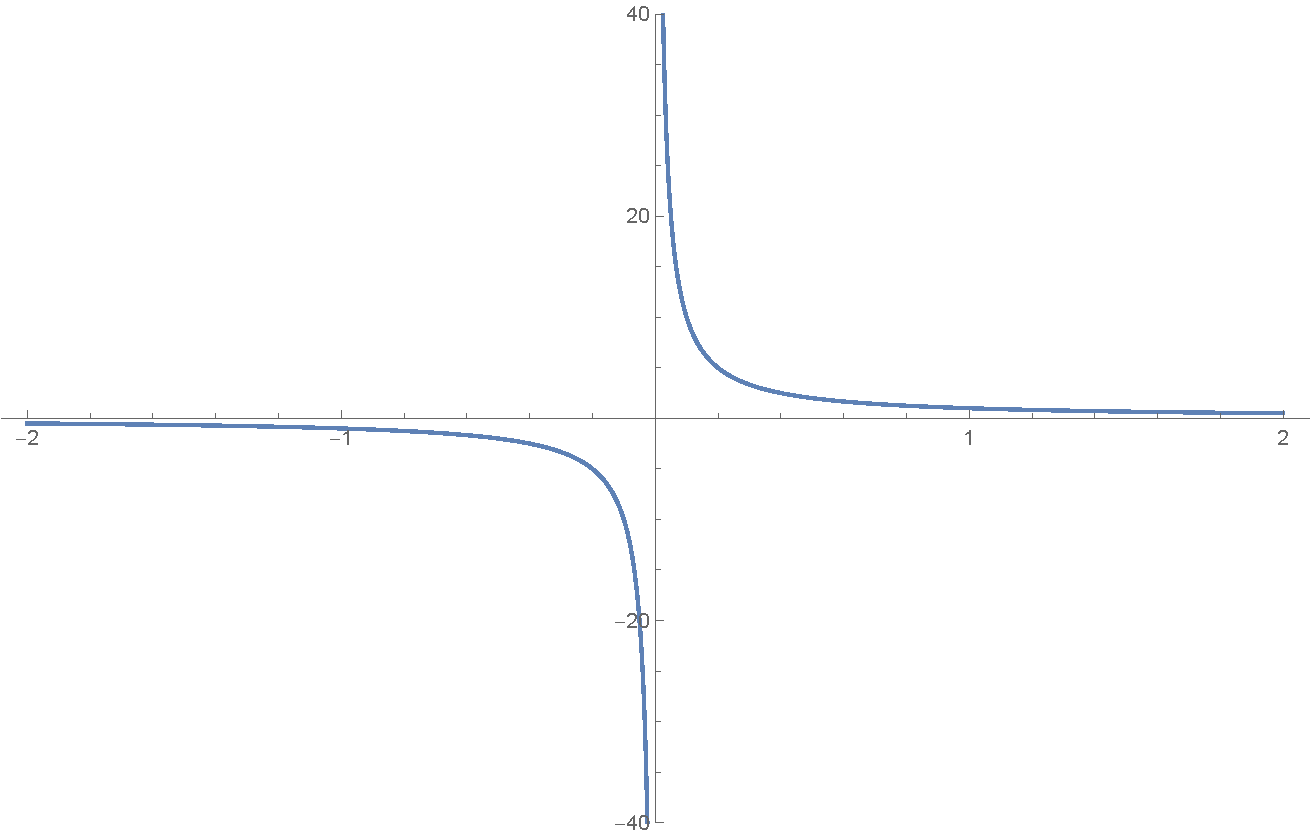
\includegraphics[height=.65\vsize]{grafy/invzero.pdf} \]
	
\end{frame}

\begin{frame}
	\frametitle{Jednostranné limity}
	Budeme se dívat na funkci jen z \uv{jedné strany}.
	\pause
	\begin{block}{Jednostranná okolí}
		Pro $c \in \R$ definujeme \emph{pravé prstencové $\varepsilon$-okolí}
		$P_+(c; \varepsilon) = (c; c+\varepsilon)$
		a \emph{levé prstencové $\varepsilon$-okolí}
		$P_-(c; \varepsilon) = (c-\varepsilon; c)$.
	\end{block}
	\pause
	\begin{alertblock}{Definice}
	Řekneme, že \emph{funkce $f$ má v bodě $c \in \R$ limitu \alert{zprava} rovnu $A \in \R^*$}, pokud platí
	\[ \textcolor{blue}{\forall \varepsilon \in \R, \varepsilon>0} \  \textcolor{red}{\exists \delta \in \R, \delta > 0}\  \textcolor{green!50!black}{\forall x \in P_{\alert+}(c; \delta)\colon f(x) \in B(A; \varepsilon)}. \]
	\end{alertblock}
	\pause
	Zapisujeme to $\lim\limits_{x \to c_{\alert+}} f(x) = A$.
\end{frame}


\begin{frame}
	\frametitle{A ještě jednou\dots}
	\pause
	\begin{alertblock}{Definice}
	Řekneme, že \emph{funkce $f$ má v bodě $c \in \R$ limitu \alert{zleva} rovnu $A \in \R^*$}, pokud platí
	\[ \textcolor{blue}{\forall \varepsilon \in \R, \varepsilon>0} \  \textcolor{red}{\exists \delta \in \R, \delta > 0}\  \textcolor{green!50!black}{\forall x \in P_{\alert-}(c; \delta)\colon f(x) \in B(A; \varepsilon)}. \]
	\end{alertblock}
	\pause
	Zapisujeme to $\lim\limits_{x \to c_{\alert-}} f(x) = A$.
\end{frame}

\section{Příklady}


\begin{frame}
	\frametitle{$\frac1x$ podruhé}
	\[ 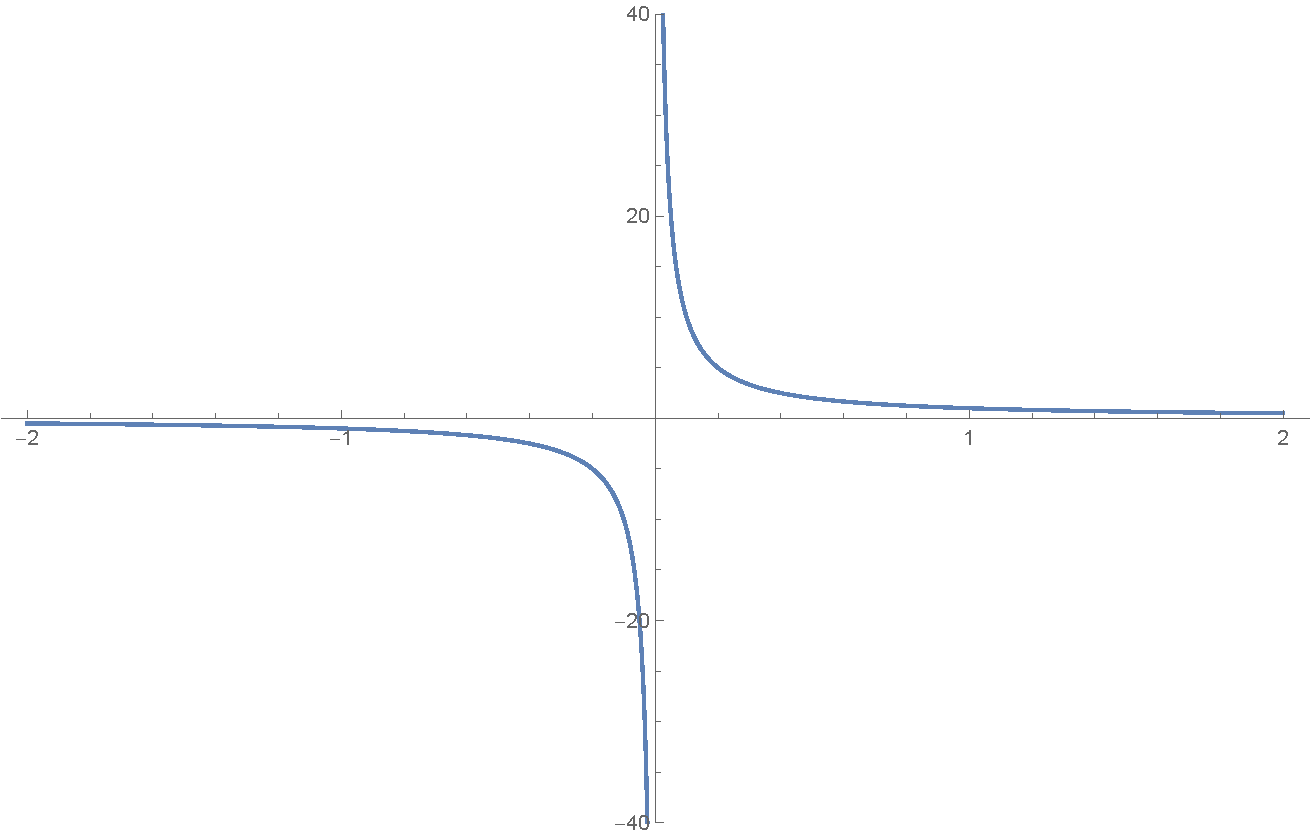
\includegraphics[height=.6\vsize]{grafy/invzero.pdf} \]
	
	\pause
	\vskip-2cm
	\[ \lim_{x \to 0_-}\frac1x = -\infty; \qquad\qquad \lim_{x \to 0_+}\frac1x = \infty. \]
	\pause
	
	\begin{center}
	(Ale $\displaystyle\lim_{x \to 0}\frac1x$ \alert{neexistuje}.)
	\end{center}
\end{frame}



\begin{frame}
		\frametitle{Tangens}
		\[ 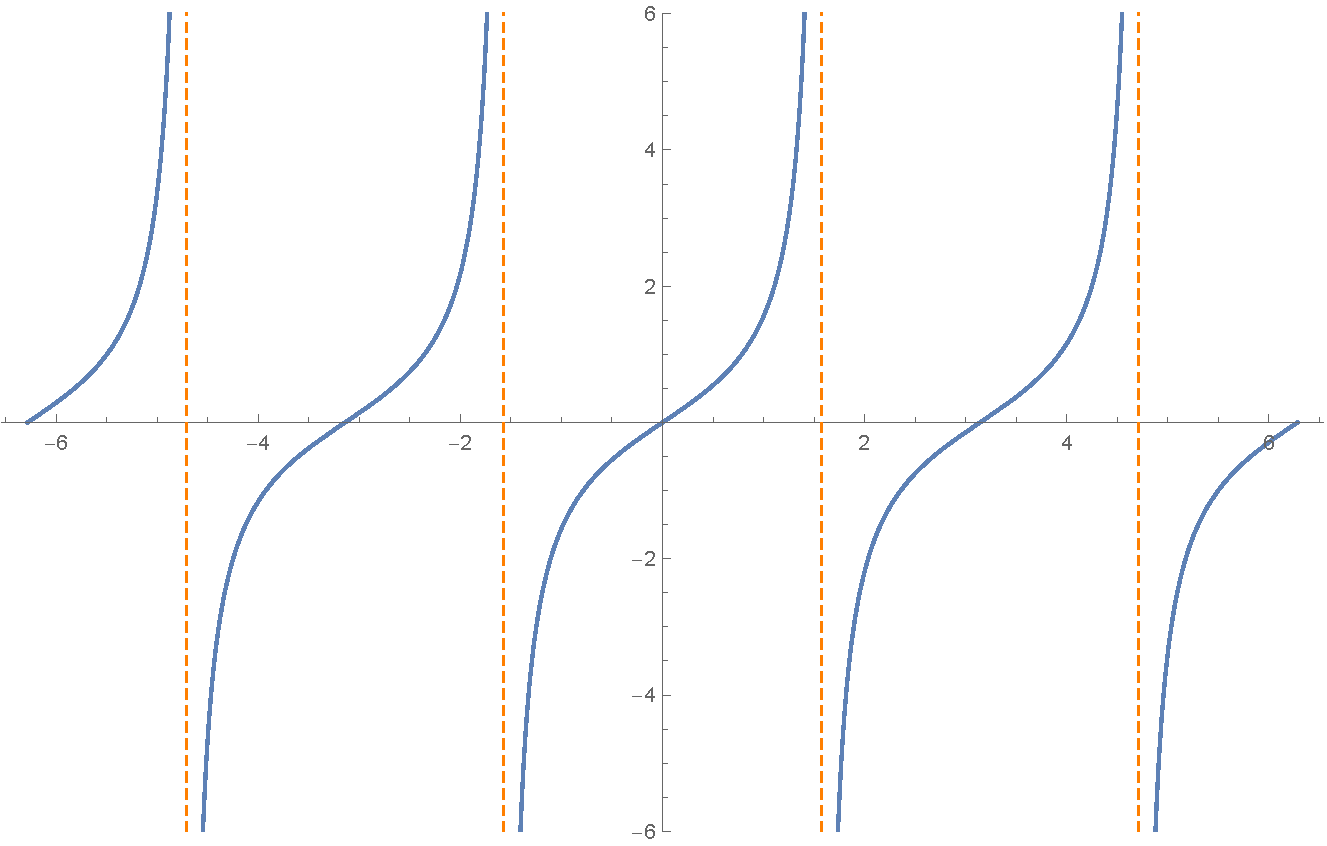
\includegraphics[height=.6\vsize]{grafy/tan.pdf} \]
		\vskip-.5cm
		\pause
		\[ \lim_{x \to \pi/2_-}\operatorname{tg}x = \infty; \quad\pause \lim_{x \to \pi/2_+}\operatorname{tg}x = -\infty; \] \pause
		%\vskip-2mm
		\[ \lim_{x \to 3\pi/2_-}\operatorname{tg}x = \infty; \quad\pause \lim_{x \to 3\pi/2_+}\operatorname{tg}x = -\infty;\]
\end{frame}


\begin{frame}
		\frametitle{Odmocnina}
		\[ 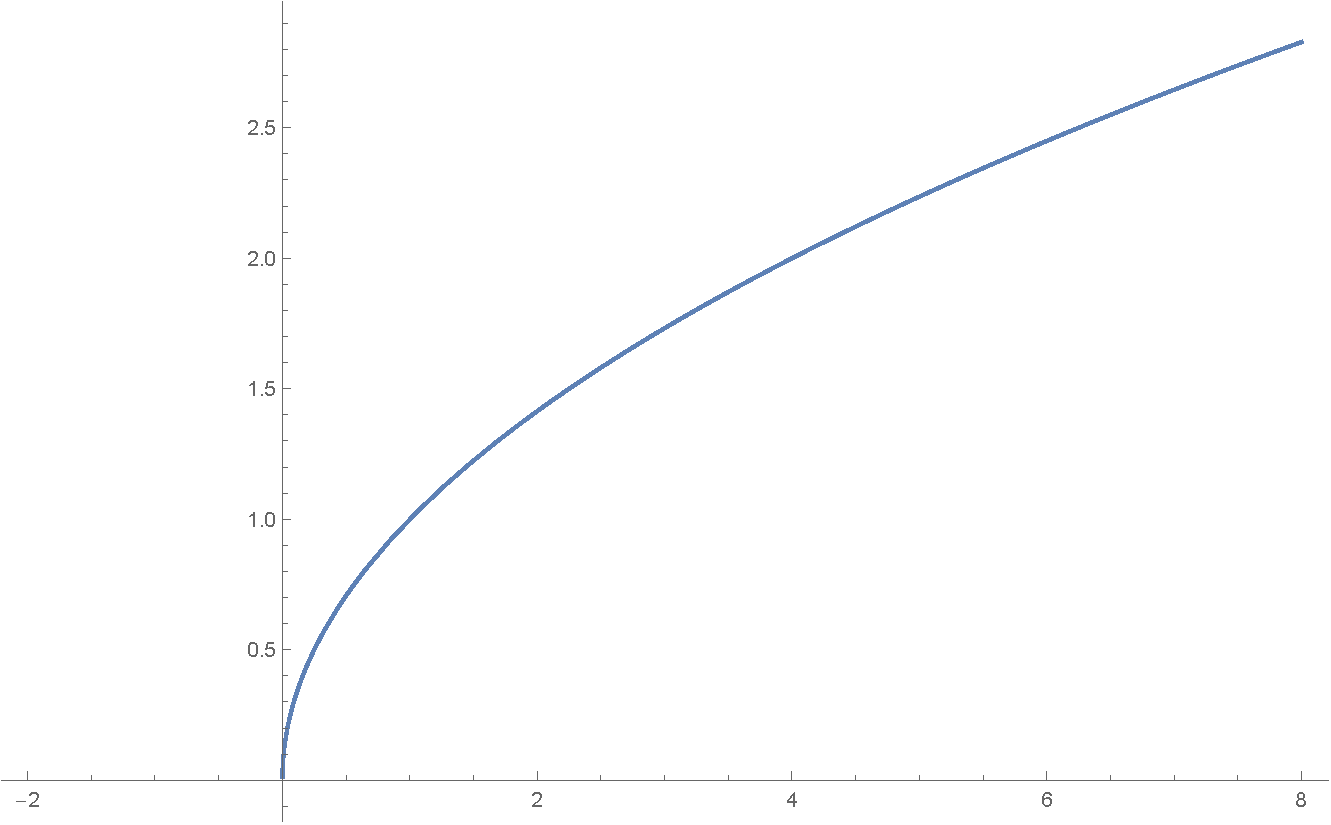
\includegraphics[height=.6\vsize]{grafy/sqrt.pdf} \]
		%\vskip-.5cm
		\pause
		\[ \lim_{x \to 0_-}\sqrt x \text{ neexistuje}; \qquad\pause \lim_{x \to 0_+}\sqrt x = 0. \]
\end{frame}


\begin{frame}
		\frametitle{$x^x$}
		\[ 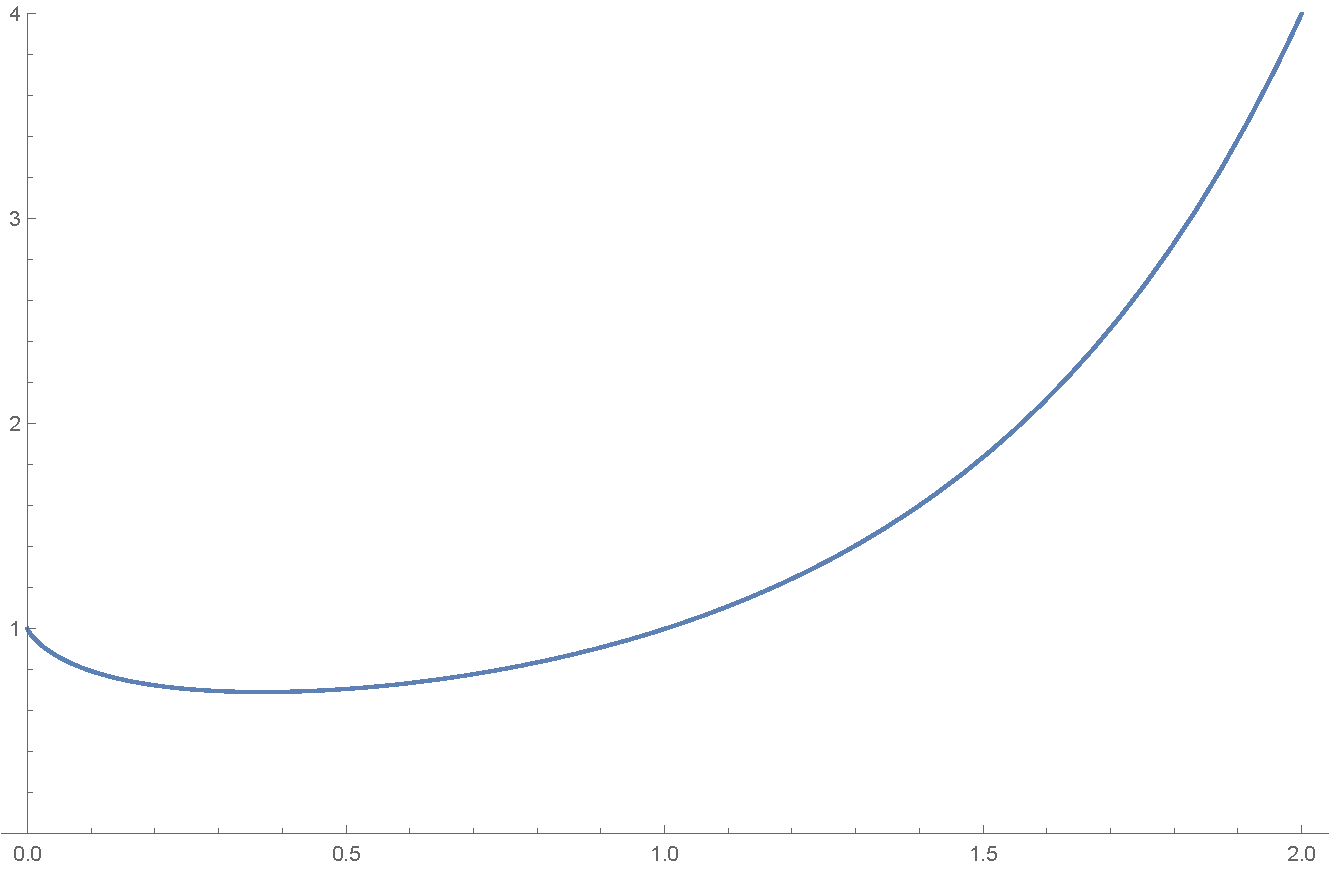
\includegraphics[height=.6\vsize]{grafy/xonx.pdf} \]
		%\vskip-.5cm
		\pause
		\[ \lim_{x \to 0_-} x^x \text{ neexistuje}; \qquad\pause \lim_{x \to 0_+} x^x = 1. \]
\end{frame}


\begin{frame}
		\frametitle{\uv{Signum}}
		\[ 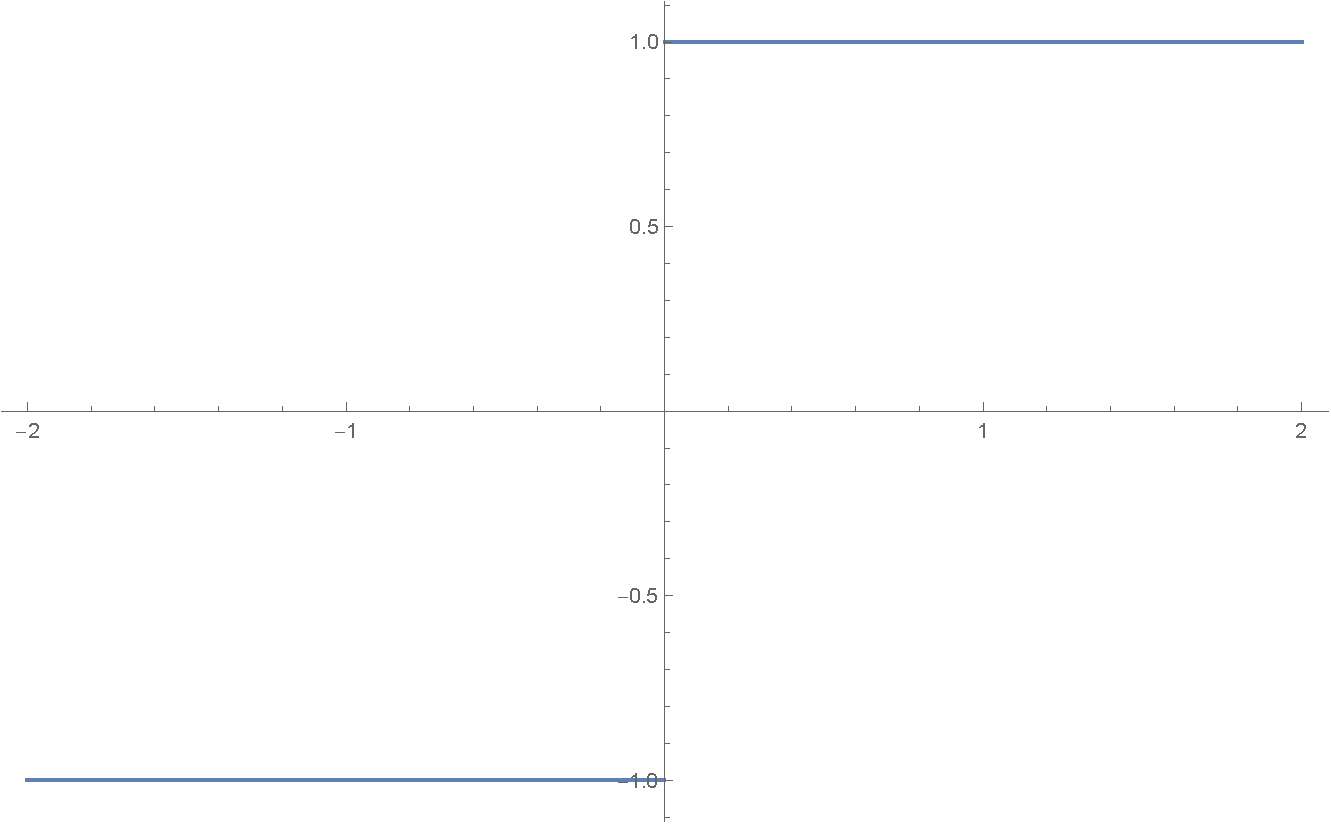
\includegraphics[height=.6\vsize]{grafy/sign.pdf} \]
		%\vskip-.5cm
		\pause
		\[ \lim_{x \to 0_-} \frac{|x|}{x} = -1; \qquad\pause \lim_{x \to 0_+} \frac{|x|}{x} = 1. \]
\end{frame}

\begin{frame}
		\frametitle{$2^{1/x}$}
		\[ 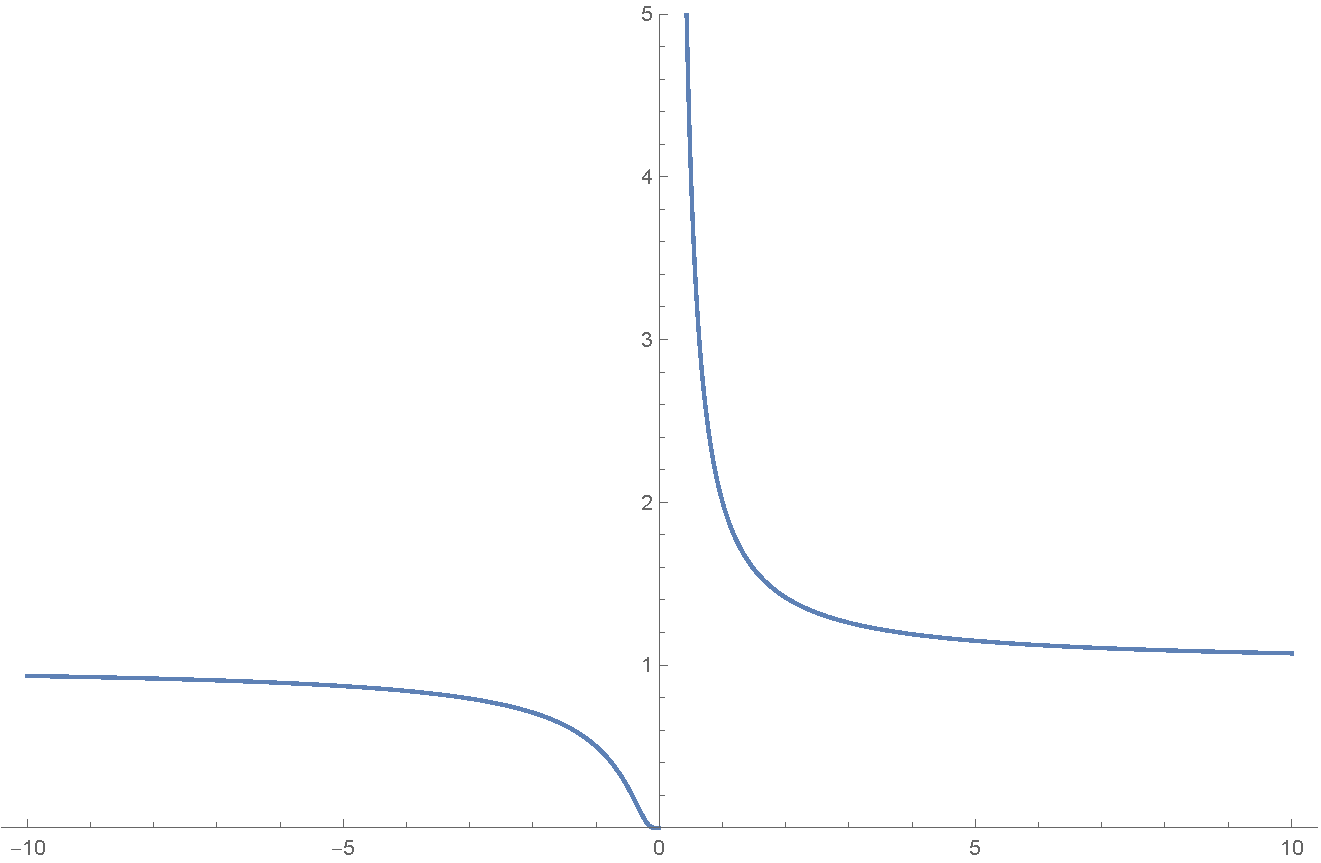
\includegraphics[height=.6\vsize]{grafy/expinv.pdf} \]
		%\vskip-.5cm
		\pause
		\[ \lim_{x \to 0_-} 2^{1/x} = 0; \qquad\pause \lim_{x \to 0_+} 2^{1/x} = \infty. \]
\end{frame}

\section{Pravidla}

\begin{frame}
		\frametitle{Vztah k běžné limitě}
		\pause
		\begin{block}{Věta}
		Funkce $f$ má v bodě $c \in \R$ (\uv{oboustrannou}) limitu $A \in \R^{*}$ právě tehdy, když má v $c$ obě jednostranné limity a ty se obě rovnají $A$.
		\end{block}
		\pause
		\[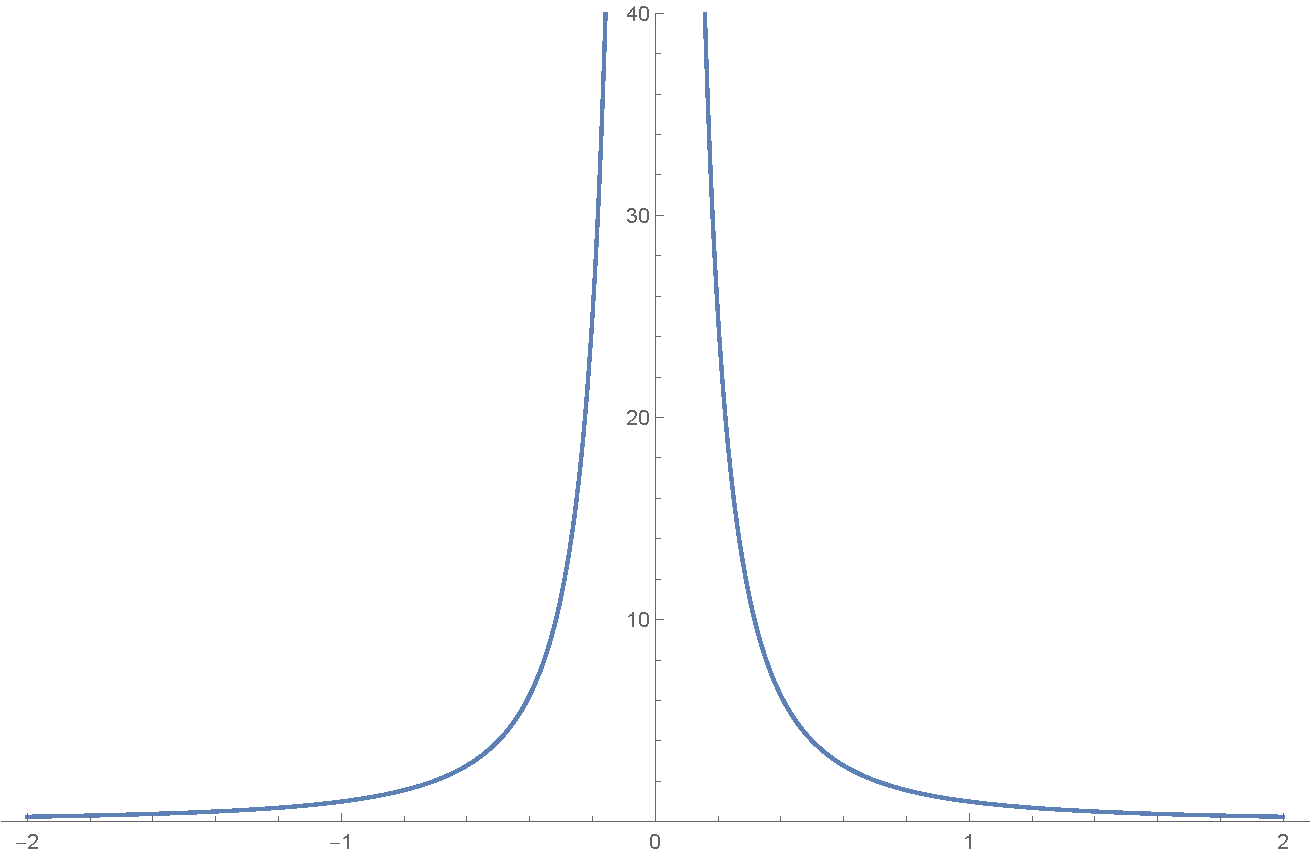
\includegraphics[height=.4\vsize]{grafy/invkvadr.pdf}\]\pause
		\[ \lim_{x \to 0_-}\frac1{x^2} = \infty \ \wedge \ \lim_{x \to 0_+}\frac1{x^2} = \infty  \pause \quad \Leftrightarrow \quad   \lim_{x \to 0}\frac1{x^2} = \infty \]	
		
\end{frame}


\begin{frame}
		\frametitle{Vztah k běžné limitě}
		%\pause
		\begin{block}{Věta}
		Funkce $f$ má v bodě $c \in \R$ (\uv{oboustrannou}) limitu $A \in \R^{*}$ právě tehdy, když má v $c$ obě jednostranné limity a ty se obě rovnají $A$.
		\end{block}
		%\pause
		\[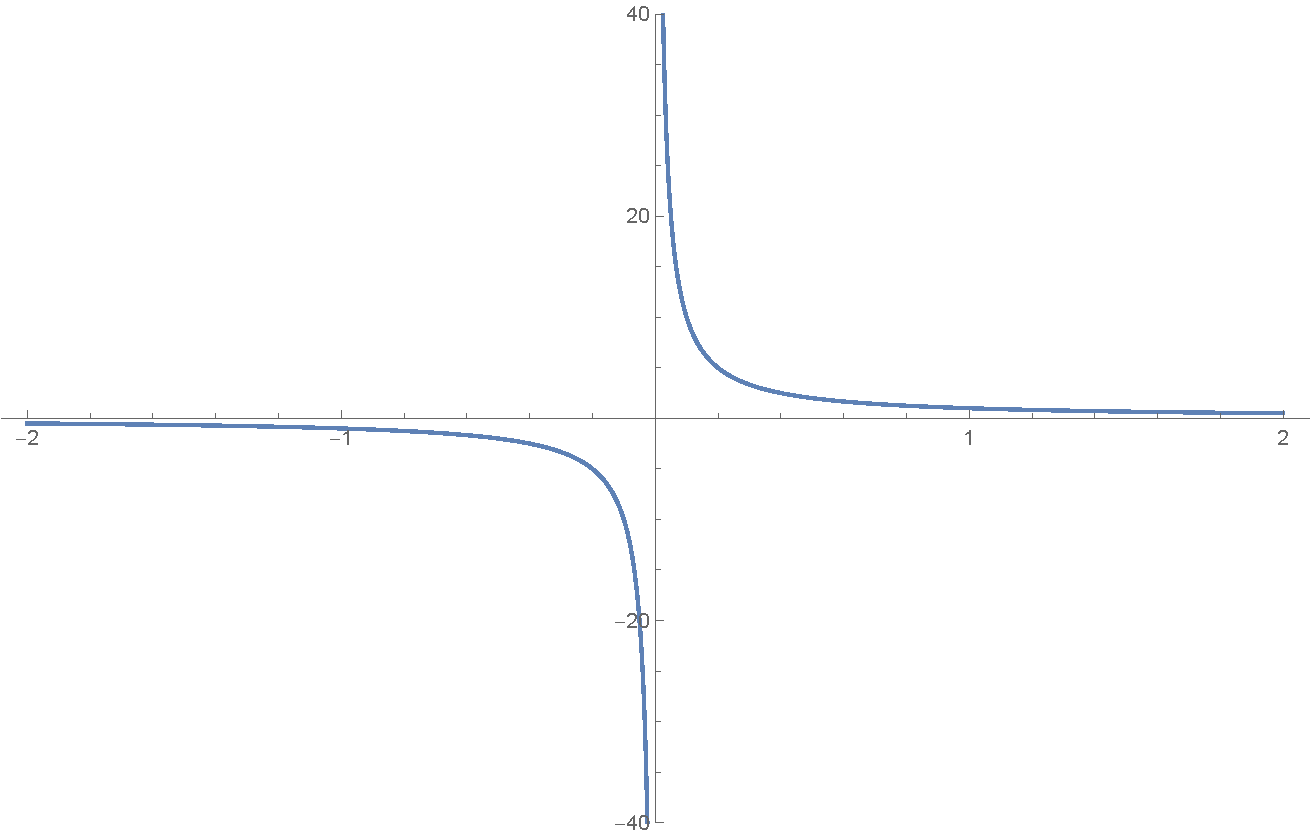
\includegraphics[height=.4\vsize]{grafy/invzero.pdf}\]\pause
		\[ \lim_{x \to 0_-}\frac1{x} = -\infty \ \wedge \ \lim_{x \to 0_+}\frac1{x} = \infty  \pause \quad \Rightarrow \quad   \lim_{x \to 0}\frac1{x} \text{ neexistuje} \]	
		
\end{frame}




\begin{frame}
		\frametitle{Počítání s limitami potřetí}
		\pause
		%Pravidla pro počítání jsou \emph{stejná} jako pro \uv{oboustranné limity}:
	Mějme dvě funkce $f$, $g$, které mají v bodě $c \in \R$ limity \alert{zprava}:
	\[ \lim_{x\to c_+}f(x) = A, \qquad \lim_{x\to c_+}g(x) = B. \]
	Potom:\pause
	\begin{itemize}
		\item Limita zprava funkce $f + g$ v bodě $c$ existuje a je rovna $A + B$, \emph{je-li $A + B$ definováno}.\pause
		\item Limita zprava funkce $f \cdot g$ v bodě $c$ existuje a je rovna $A \cdot B$,  \emph{je-li $A\cdot B$ definováno}.\pause
		\item Limita zprava funkce $\frac fg$ v bodě $c$ existuje a je rovna $\frac AB$,  \emph{je-li $\frac AB$ definováno}.%\pause
	\end{itemize}
	\pause
	Symbolicky:
	\vskip-8mm \scriptsize
	\begin{align*}
	\lim_{x \to c_+}(f(x) + g(x)) &= \lim_{x \to c_+}f(x) + \lim_{x \to c_+}g(x),\\
	\lim_{x \to c_+}(f(x) \cdot g(x)) &= \bigl(\lim_{x \to c_+}f(x)\bigr) \cdot \bigl(\lim_{x \to c_+}g(x)\bigr),\\
	\lim_{x \to c_+}\frac{f(x)}{g(x)} &= \frac{\lim\limits_{x \to c_+}f(x)}{\lim\limits_{x \to c_+}g(x)}
	\end{align*}
		
\end{frame}


\begin{frame}
		\frametitle{Počítání s limitami počtvrté}

		%Pravidla pro počítání jsou \emph{stejná} jako pro \uv{oboustranné limity}:
	Mějme dvě funkce $f$, $g$, které mají v bodě $c \in \R$ limity \alert{zleva}:
	\[ \lim_{x\to c_-}f(x) = A, \qquad \lim_{x\to c_-}g(x) = B. \]
	Potom: 
	\begin{itemize}
		\item Limita zleva funkce $f + g$ v bodě $c$ existuje a je rovna $A + B$,   \emph{je-li $A + B$ definováno}. 
		\item Limita zleva funkce $f \cdot g$ v bodě $c$ existuje a je rovna $A \cdot B$,   \emph{je-li $A\cdot B$ definováno}. 
		\item Limita zleva funkce $\frac fg$ v bodě $c$ existuje a je rovna $\frac AB$,   \emph{je-li $\frac AB$ definováno}.% 
	\end{itemize}
	 
	Symbolicky: 
	\vskip-8mm \scriptsize
	\begin{align*}
	\lim_{x \to c_-}(f(x) + g(x)) &= \lim_{x \to c_-}f(x) + \lim_{x \to c_-}g(x),\\
	\lim_{x \to c_-}(f(x) \cdot g(x)) &= \bigl(\lim_{x \to c_-}f(x)\bigr) \cdot \bigl(\lim_{x \to c_-}g(x)\bigr),\\
	\lim_{x \to c_-}\frac{f(x)}{g(x)} &= \frac{\lim\limits_{x \to c_-}f(x)}{\lim\limits_{x \to c_-}g(x)}
	\end{align*}
		
\end{frame}


\end{document}
